\documentclass[usenames,dvipsnames,tikz]{standalone}
\usetikzlibrary{patterns}
%\usepackage{tikz}
%\usepackage{standalone}
\begin{document}
	
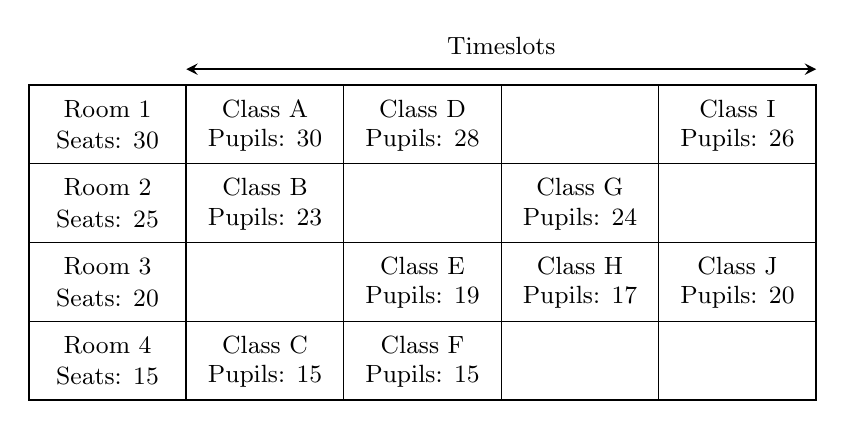
\begin{tikzpicture}
%\draw [help lines] (-1,-2) grid (13,11);


%------------------------------

\draw [thick] (0,0) rectangle (10,4);

\draw [thick, <->, >=stealth] (2,4.2) -- (10,4.2);
\node at (6,4.5) {\small Timeslots};

\draw [thick] (2,0) -- (2,4);
\draw (4,0) -- (4,4);
\draw (6,0) -- (6,4);
\draw (8,0) -- (8,4);

\draw (0,1) -- (10,1);
\draw (0,2) -- (10,2);
\draw (0,3) -- (10,3);

\node at (1,3.7) {\small Room 1};
\node at (1,3.3) {\small Seats: 30};

\node at (1,2.7) {\small Room 2};
\node at (1,2.3) {\small Seats: 25};

\node at (1,1.7) {\small Room 3};
\node at (1,1.3) {\small Seats: 20};

\node at (1,0.7) {\small Room 4};
\node at (1,0.3) {\small Seats: 15};

\node at (3,3.7) {\small Class A};
\node at (3,3.3) {\small Pupils: 30};

\node at (3,2.7) {\small Class B};
\node at (3,2.3) {\small Pupils: 23};

\node at (3,0.7) {\small Class C};
\node at (3,0.3) {\small Pupils: 15};

\node at (5,3.7) {\small Class D};
\node at (5,3.3) {\small Pupils: 28};

\node at (5,1.7) {\small Class E};
\node at (5,1.3) {\small Pupils: 19};

\node at (5,0.7) {\small Class F};
\node at (5,0.3) {\small Pupils: 15};

\node at (7,2.7) {\small Class G};
\node at (7,2.3) {\small Pupils: 24};

\node at (7,1.7) {\small Class H};
\node at (7,1.3) {\small Pupils: 17};

\node at (9,3.7) {\small Class I};
\node at (9,3.3) {\small Pupils: 26};

\node at (9,1.7) {\small Class J};
\node at (9,1.3) {\small Pupils: 20};






\end{tikzpicture}
	
\end{document}